\chapter{Robot User Guide}
\label{app:robotuserguide}
\lhead{Appendix \ref{app:robotuserguide}. \emph{Robot User Guide}}

In this section, the basic operation of the completed \textit{ExplorerBot} robot hardware is outlined. An annotated diagram of the completed robot design is shown in Figure \ref{fig:robotoutlineannotated} below.

\begin{figure}[H]
	\centering
		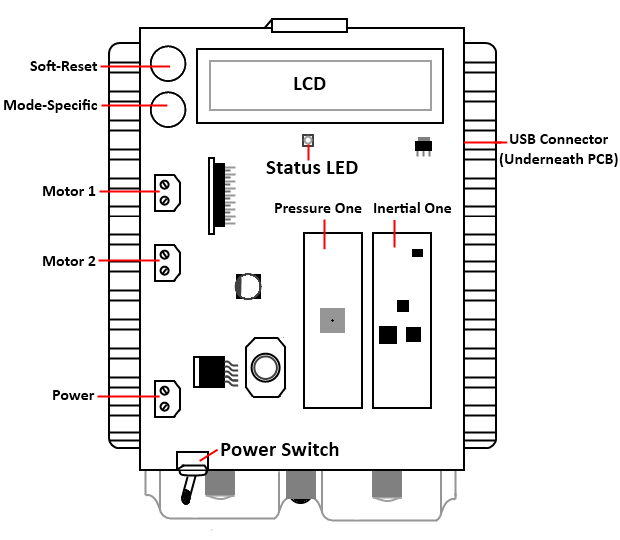
\includegraphics[width=120mm]{RobotOutlineAnnotated.png}
	\rule{35em}{0.5pt}
	\caption[Annotated diagram of the robot]{Annotated diagram of the robot.}
	\label{fig:robotoutlineannotated}
\end{figure}

\section{Power Requirements}

The robot requires a 6-9V DC input power supply, capable of supplying up to 1A of current. Ideally, a 7.2V Lithium Ion battery should be used for this purpose for maximum operating time (due to its abilitiy to supply large amount of instataneous current, used by the motors when switched on).

\section{Supported USB Devices}

Several classes of USB devices are supported by the robot firmware. Where possible, each class is supported in a generic manner, so that any device compliant with the relevant USB class specification can be used.

\subsection{HID Class Devices}

For robot control over a wired interface, USB HID class devices may be inserted into the robot's USB recepticle. Compatible HID devices must contain at least one four-way directional pad and four buttons for all robot features to be operational. The button mappings are listed in Table \ref{tab:robotbuttonmappings} below.

\begin{table}[H]
	\begin{center}
		\begin{tabular}{ | l | l | l |}
			\hline
			\textbf{Function}		& \textbf{PS3 Controller}	& \textbf{Other HID Device} \\ \hline

			Left					& D-Pad Left				& Button 1	\\ \hline
			Forward					& D-Pad Up					& Button 2	\\ \hline
			Backward				& D-Pad Down				& Button 3	\\ \hline
			Right					& D-Pad Right				& Button 4	\\ \hline
			Headlights (Momentary)	& R2						& Button 5	\\ \hline
			Horn					& L2						& Button 6	\\ \hline
			Headlights (Toggle)		& R1						& Button 7	\\ \hline
			Novelty Horn			& L1						& Button 8	\\ \hline

		\end{tabular}
		\caption[USB HID Robot Button Mappings]{Button mappings between various USB HID devices and the robot functions.}
		\label{tab:robotbuttonmappings}
	\end{center}
\end{table}

In the special case of a Playstation 3 controller being inserted into the robot, the controller will be automatically configured to pair over Bluetooth with the address of the last Bluetooth USB adapter inserted into the robot. Once paired, the controller may then establish a connection with the robot over Bluetooth by pressing the PS3 button located in the center of the controller.

\subsection{Mass Storage Class Devices}

Flash drives suitably formatted with a FAT32 filesystem may be used for sensor logging and system configuration of the robot. Compatible memory sticks must be no more than 4GB in size.

On insertion, the robot will attempt to read a file names \texttt{REMADDR.TXT} from the disk. This file should contain the Bluetooth Device Address of the remote device the robot should attempt to establish a connection with while in Bluetooth mode. 

\subsection{Bluetooth Adapter Devices}

% TODO

\section{Supported Bluetooth Services}

% TODO

\subsection{HID Service}

% TODO

\subsection{RFCOMM Service}

% TODO